\section{AutoPreprocessing Module}
\subsection{Experimental Setup}

\paragraph{Experimental Environment}\par

All experiments were implemented in Python using Pandas, NumPy, and Scikit-learn for tabular data processing and model evaluation. AutoCleanML was used as the baseline preprocessing framework, while Accelera was used as the proposed automated preprocessing system. The experiments were executed under identical conditions.

\paragraph{Datasets}\par

A total of 16 tabular datasets were used, collected from Kaggle. The datasets include both classification and regression tasks with varying sizes and feature complexities.

\begin{table}[H]
\centering
\caption{Summary of Datasets Used in Experiments}
\begin{tabular}{|l|c|c|}
\hline
\textbf{Dataset} & \textbf{Shape} & \textbf{Task Type} \\
\hline
startup\_founder\_burnout\_2026 & (50000, 29) & Classification \\
healthy\_diet\_calorie\_intake & (6000, 15) & Classification \\
ai\_student & (50000, 16) & Classification \\
gaming\_addiction & (250, 49) & Classification \\
Teen\_Mental\_Health\_Dataset & (1200, 13) & Classification \\
student\_exam\_performance\_dataset & (10000, 17) & Classification \\
heart & (302, 14) & Classification \\
Dataset\_spine & (310, 7) & Classification \\
diabetes\_dataset & (100000, 31) & Classification \\
student\_placement\_synthetic & (100000, 18) & Classification \\
Titanic-Dataset & (891, 12) & Classification \\
customer\_purchase\_data & (1388, 9) & Classification \\
global\_ai\_jobs & (90000, 35) & Regression \\
CarPrice\_Assignment & (205, 26) & Regression \\
Concrete\_Data\_Yeh & (1005, 9) & Regression \\
Housing & (545, 13) & Regression \\
\hline
\end{tabular}
\end{table}

\paragraph{Compared Frameworks}\par

Two preprocessing tools were evaluated:

\textbf{AutoCleanML}: A fully automated data cleaning AutoCleanML Python library, that performs missing value handling, encoding, and feature preparation.

\textbf{Accelera}: A proposed automated preprocessing tools supporting tabular, image, and text data, with additional reporting and visualization capabilities.

\paragraph{Preprocessing Configuration}

Identical experimental settings were used across both tools. A validation size of 20\% and a random state of 42 were applied for all datasets. For classification tasks, stratified sampling was used to preserve class distribution.

Apart from specifying the target column and excluding unnecessary columns when required, all preprocessing parameters were kept at their default values for both frameworks.
\paragraph{Results and Discussion}

\subparagraph{Classification Results}\par

The performance of both frameworks was evaluated on multiple classification datasets using F1-macro score as the evaluation metric.

\begin{figure}[H]
    \centering
    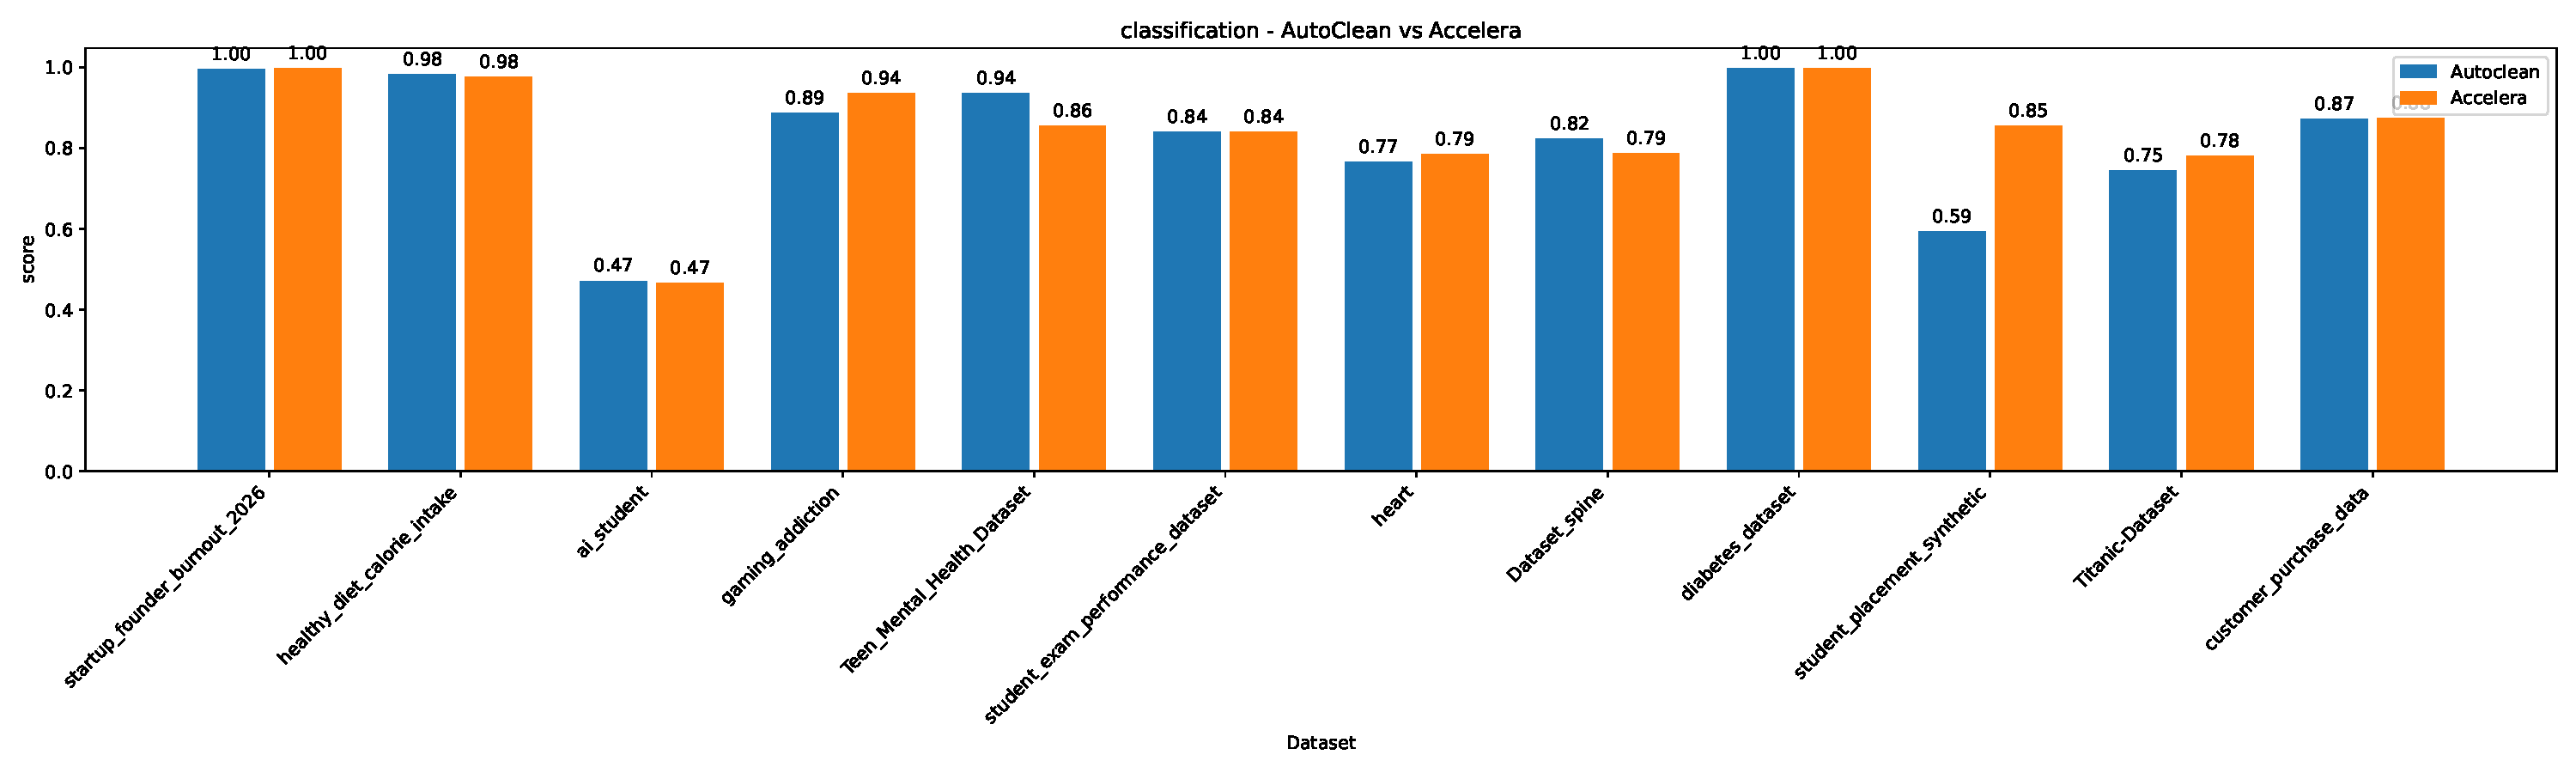
\includegraphics[width=\textwidth,height=0.3\textheight]{imgs/tabular_dataset_comparison_classification_score}
    \caption{Classification Performance Comparison (F1-Macro Score)}
\end{figure}


\begin{figure}[H]
    \centering
    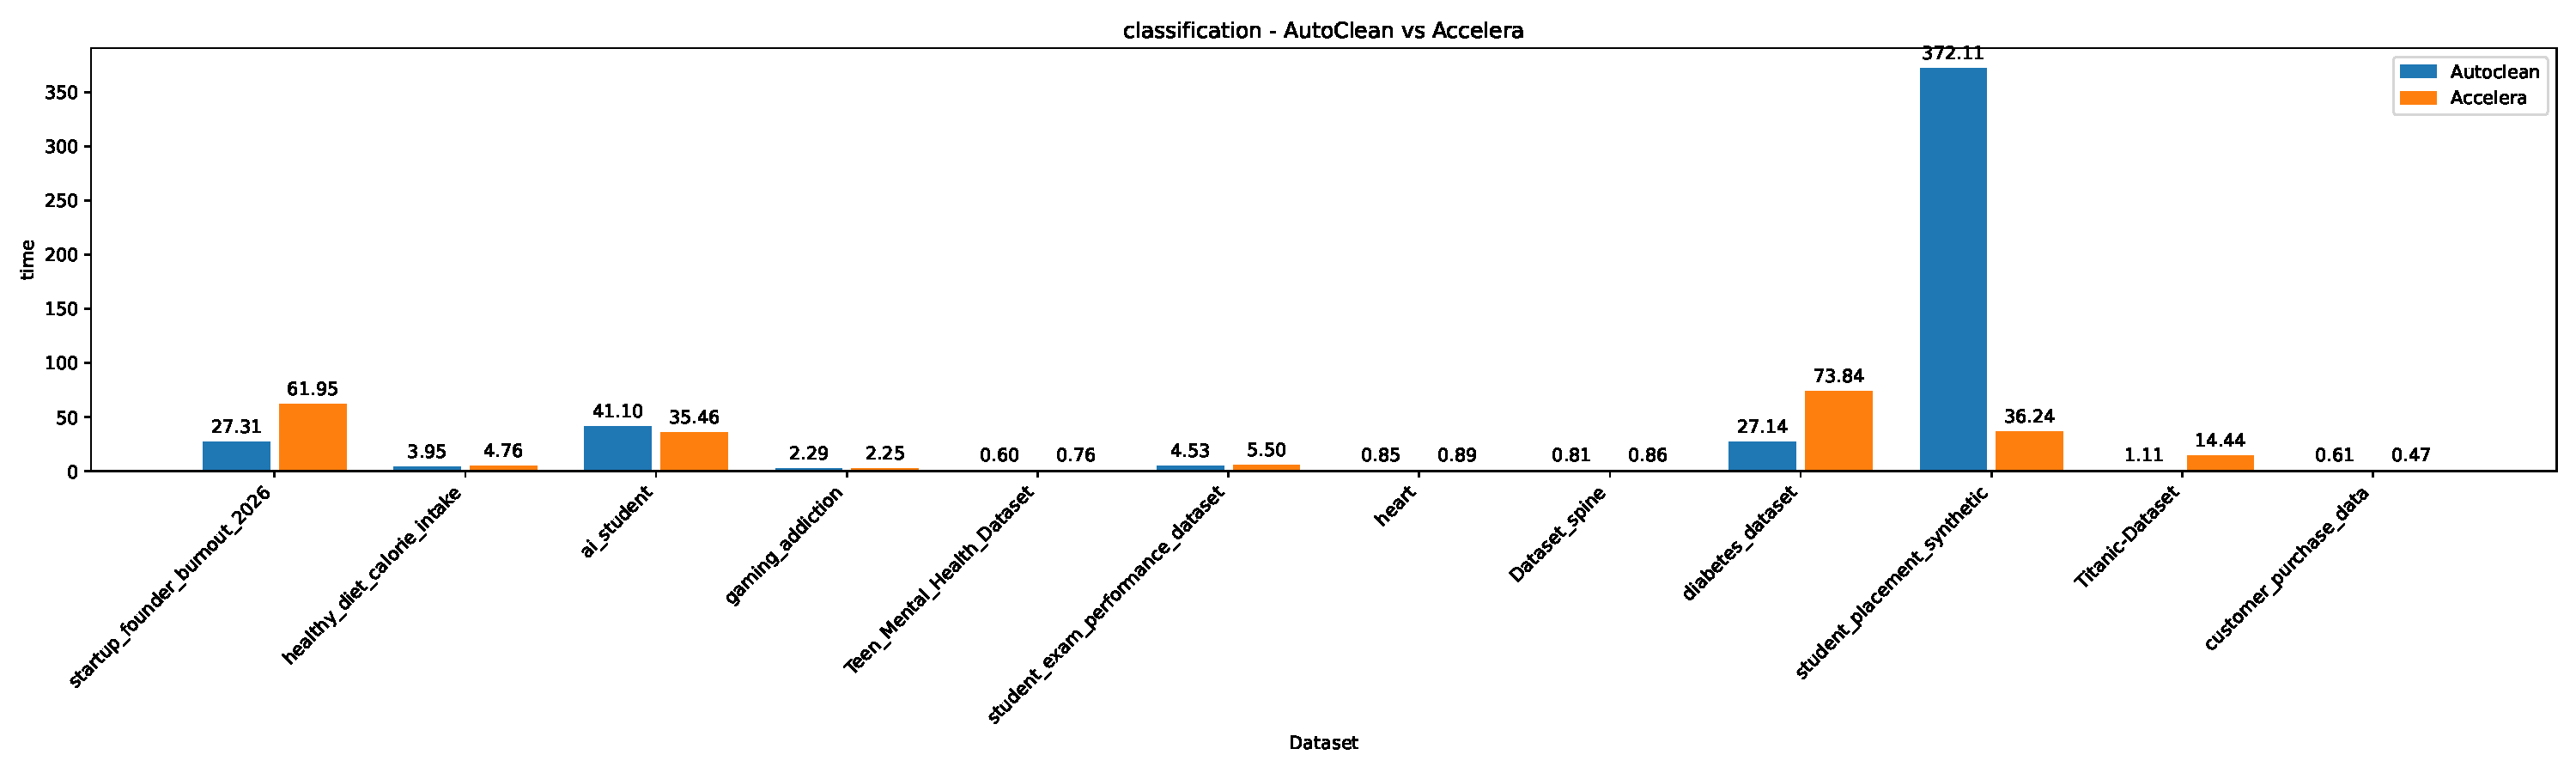
\includegraphics[width=\textwidth,height=0.3\textheight]{imgs/tabular_dataset_comparison_classification_time}
    \caption{Classification Preprocessing Time Comparison}
\end{figure}

\subparagraph{Regression Results}

Regression performance was evaluated using the R$^2$ score.

\begin{figure}[H]
    \centering
    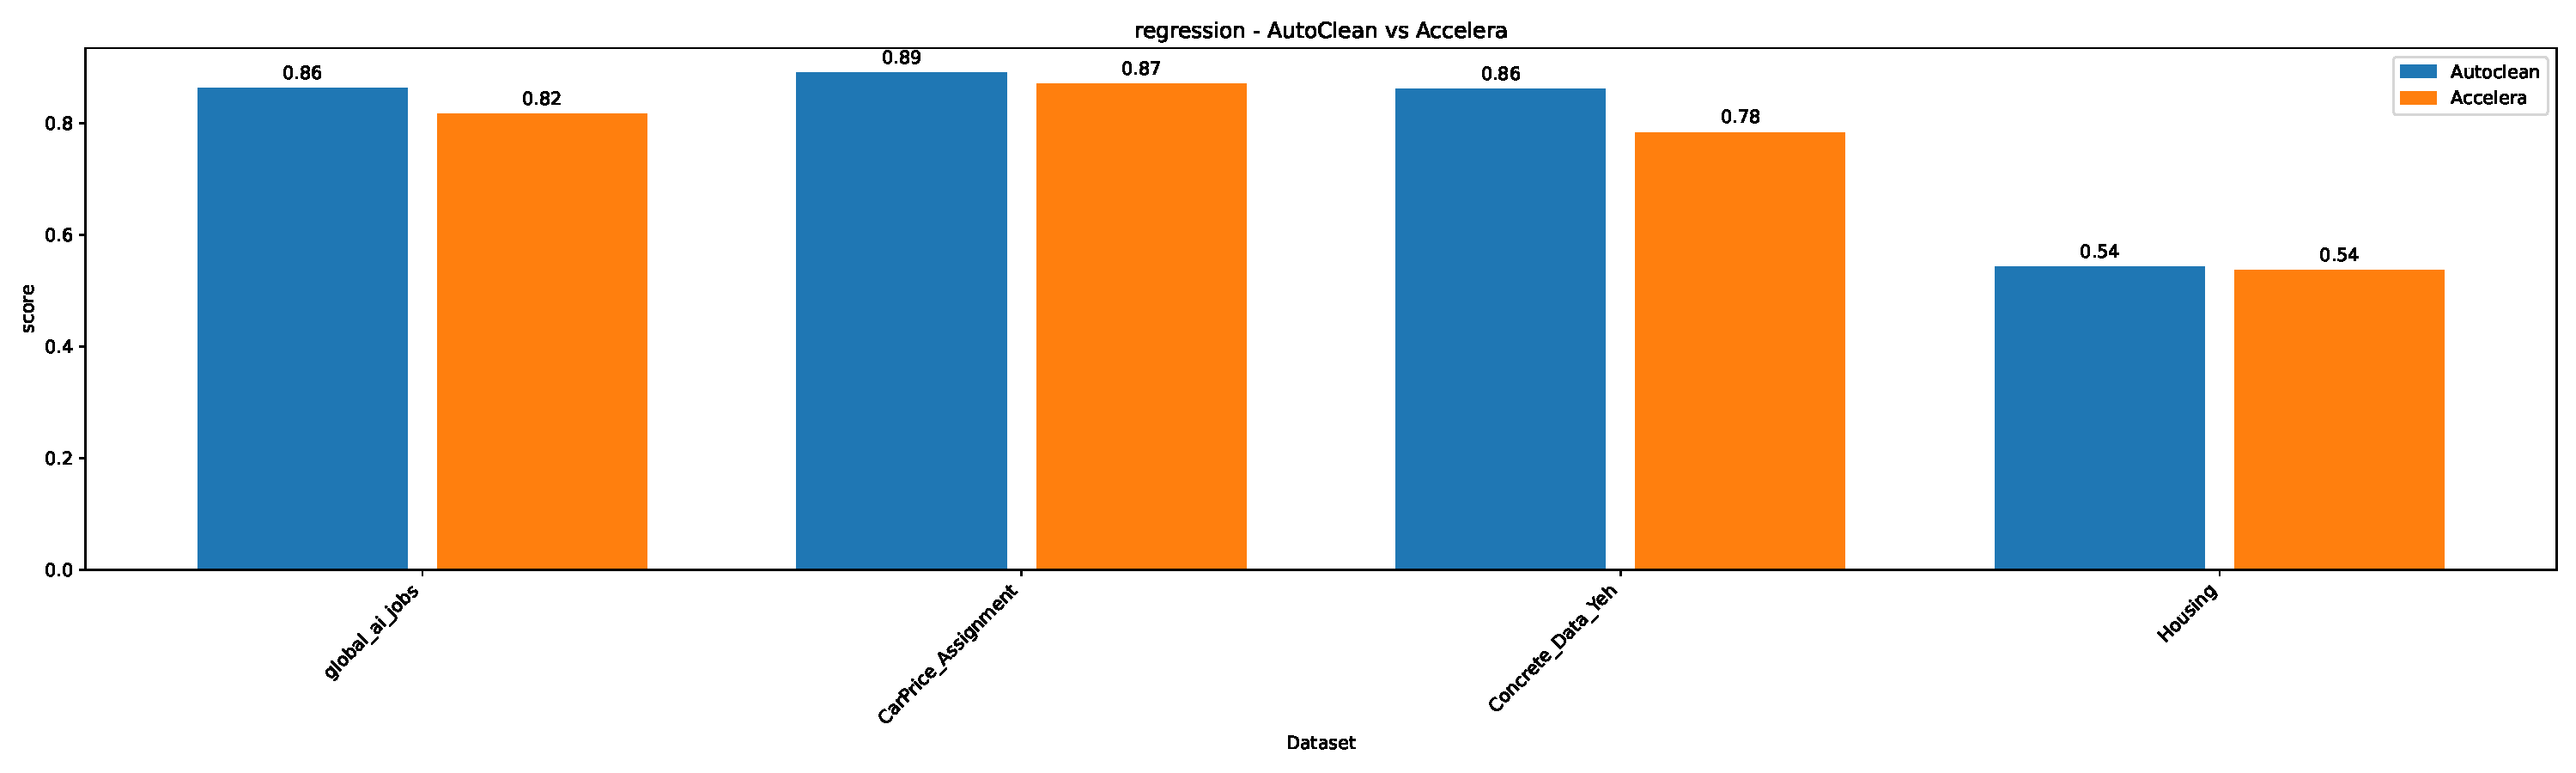
\includegraphics[width=\textwidth,height=0.3\textheight]{imgs/tabular_dataset_comparison_regression_score}
    \caption{Regression Performance Comparison (R$^2$ Score)}
\end{figure}


\begin{figure}[H]
    \centering
    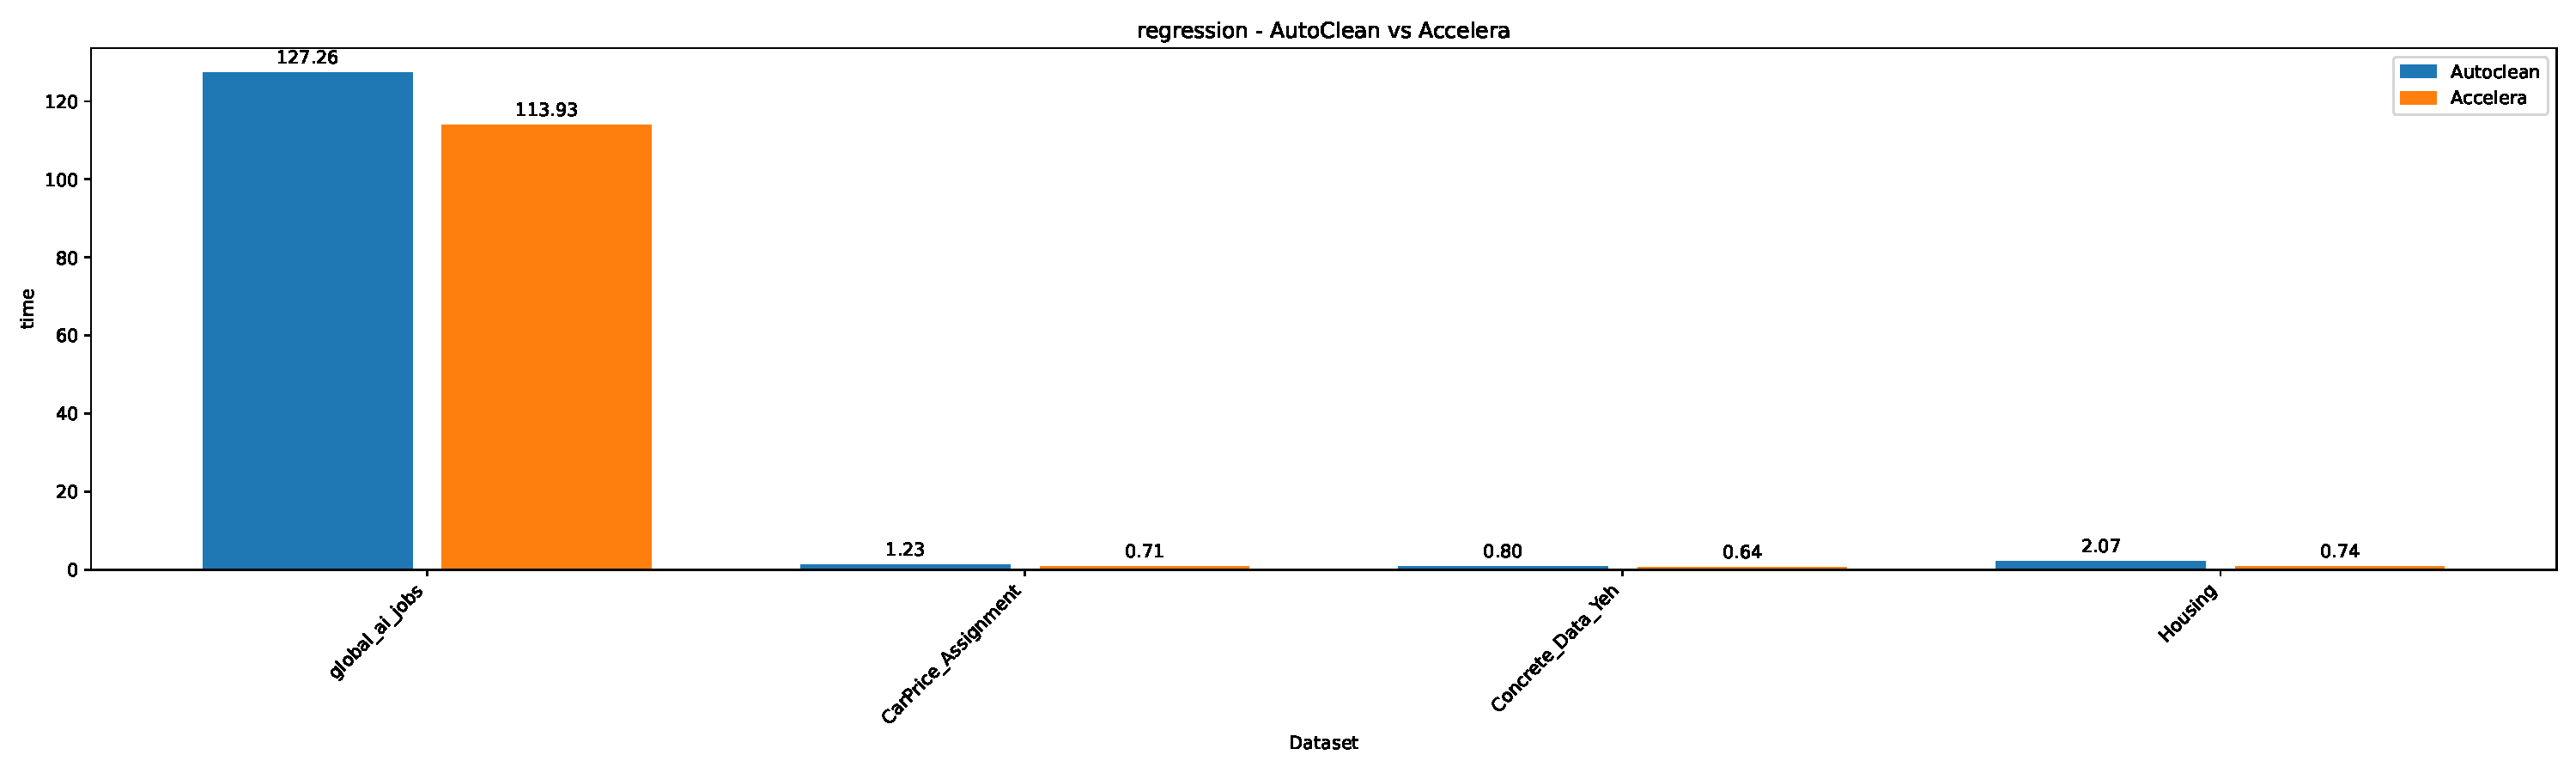
\includegraphics[width=\textwidth,height=0.3\textheight]{imgs/tabular_dataset_comparison_regression_time}
    \caption{Regression Preprocessing Time Comparison}
\end{figure}
